\chapter{Unit Testing}

\section{Analyse und Begründung für Umfang der Tests}

Um die Funktionalität der einzelnen Komponenten gewährleisten zu können werden Unit-Tests eingesetzt.
Dabei werden für die einzelnen Tests nur die, für diesen Test, relevanten Teile des Systems verwendet.
Da Abhängigkeiten zu anderen Komponenten die Tests nicht beeinflussen sollen werden alle anderen Komponenten durch Fake-/Mock-Objekte ersetzt.
Das Zusammenspiel mit den anderen Komponenten kann in Integrationstests getestet werden.
Außerdem tragen Unit-Tests auch zur Dokumentation bei, indem das gewünschte Verhalten der Komponente für Regel- und Ausnahmefälle in den Testfällen dokumentiert ist.
\newline
Für dieses Projekt wird \textit{JUnit} als Framework für die Erstellung und Ausführung von Java-Unit-Tests verwendet.
Bei der Implementierung der Tests wurde darauf geachtet die ATRIP-Regeln (\textit{Automatic, Thorough, Repeatable, Independent, Professional}) möglichst zu beachten.
\newline
Teile des Codes in diesem Projekt werden für Android-Spezifische UI-Aufgaben benötigt und können deshalb nur schlecht getestet werden. Das führt auch dazu, dass die Code-Coverage über das gesamte Projekt vergleichsweise klein sein kann und in diesem Fall keine sinnvolle Aussage über die Genauigkeit der Tests ermöglicht.
Stattdessen sollte hier zur Beurteilung der Testabdeckung nur die Code-Coverage der nicht-UI-Klassen betrachtet werden.
\newline
Allgemein wird darauf verzichtet triviale Funktionen, wie zum Beispiel Getter zu testen.
Tests dieser Funktionen würden bei großem Aufwand nur einen minimalen Mehrwert bringen, da keine echte Funktionalität getestet wird.
Stattdessen sollen sich die Tests auf relevante Funktionalität des Systems fokussieren.
Das bedeutet, dass vor allem die Klassen getestet werden sollen, die häufig verwendet werden und auch die Klassen, die für die Funktion der Anwendung unerlässlich sind.
UI-Klassen, die aufgrund starker Abhängigkeiten zu Android-Klassen schwer testbar sind sollen weniger ausführlich getestet werden.
\newline
Für die Tests innerhalb dieses Systems wurden drei Kernfunktionalitäten identifiziert, die von einer hohen Testabdeckung am stärksten profitieren.
Diese sind das Abrufen von Daten von der API, die Konvertierung von API-Datentypen zu Datentypen der Anwendung und in diesem Zusammenhang auch das Caching von abgerufenen Daten um die Netzwerklast zu reduzieren.
\newline
Diese Funktionalitäten verteilen sich auf die Packages \textit{client}, \textit{data} und \textit{repository}.
Abbildung \hyperref{fig:Code_Coverage} zeigt einen Code-Coverage-Report dieser Packages (Stand: Commit \href{https://github.com/lukaspanni/OpenSourceStats/tree/ac3c4098d8f89f5eed7142d675ca49c4d3dd724f}{ac3c409}).
\begin{figure}[h]
  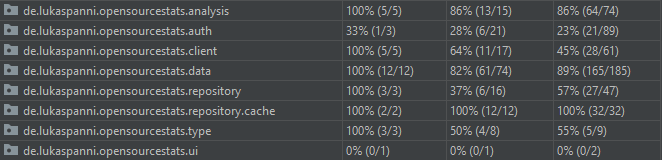
\includegraphics{Code_Coverage.png}
  \centering
  \caption{Code Coverage Report}
  \label{fig:Code_Coverage}
\end{figure}
Der Code-Coverage-Report, zeigt, dass alle relevanten Klassen getestet wurden.
Allerdings fällt dabei auf, dass die Coverage der einzelnen Methoden unterschiedlich ist, was darauf zurückzuführen ist, dass versucht wurde, triviale Funktionalität nicht ausführlich zu testen.
Im Folgenden werden Funktionalität und Tests der einzelnen Packages noch weiter erläutert.
\newline
\newline
Das data-Package enthält alle Klassen, die als Nutzdaten von der Anwendung verarbeitet werden.
Antworten, die von der API empfangen werden, werden in einem ersten Schritt in einen solchen Datentyp konvertiert.
Diese Konvertierungen werden in den Konstruktoren der Klassen durchgeführt. Ansonsten werden diese Klassen hauptsächlich zur Speicherung von Anwendungsdaten verwendet und enthalten nur vergleichsweise wenig weitere Funktionalität.
Da die Konvertierung von API-Datentyp in Anwendungsdatentyp sehr häufig verwendet wird und die Anwendungsdatentypen generell an vielen verschiedenen verwendet werden, sind hier  ausführliche Tests notwendig.
Der Fokus der Tests liegt dabei auf den Konstruktoren, die wenigen weiteren Funktionalitäten der Klassen sind weniger wichtig und meist trivial.
Die Code-Coverage von 79\% aller Methoden wird deshalb als gut angesehen, vor allem wenn die Line-Coverage von 88\% in die Betrachtung mit einbezogen wird.
\newline
\newline
Im repository-Package, sind einerseits Repository-Klassen enthalten, die den Zugriff auf Anwendungsdaten abstrahieren und dabei das Caching der Daten transparent machen.
Andererseits finden sich hier auch die Klassen, die für die Umsetzung des Cachings verwendet werden.
Die Repository-Klassen übernehmen die Funktion, die Daten aus dem Cache abzurufen, wenn diese dort vorhanden sind und ansonsten die Daten über Funktionalität, die im client-Package implementiert ist von der API-abzurufen.
Als zentrale Komponente, um auf Daten zuzugreifen sind die Repository-Klassen deshalb  entscheidend für die Funktionalität der gesamten Anwendung.
Aus diesem Grund ist es wichtig hier eine möglichst hohe Testabdeckung zu erreichen.
Die niedrige Method-Coverage von nur 42\% ist hier trotzdem gut zu bewerten, da sie auf nicht getestete triviale Funktionen zurückzuführen ist.
Diese trivialen Funktionen sind verschieden Parametrisierte Konstruktoren und Hilfsfunktionen, die selbst wiederum nur Standard-Parameter für getestete Funktionen bereitstellen (siehe: \href{https://github.com/lukaspanni/OpenSourceStats/blob/ac3c4098d8f89f5eed7142d675ca49c4d3dd724f/app/src/main/java/de/lukaspanni/opensourcestats/repository/UserContributionsRepository.java#L51-L65}{UserCotributionsRepository.load...})
\newline
Die Komponente zum Caching ist ebenfalls wichtig, da ohne funktionierendes Caching sehr viele Anfragen über das Netzwerk gesendet werden müssen, was nicht nur die Menge der übertragenen Daten unnötig erhöht, sondern auch die Reaktionszeit der Anwendung verschlechtert.
Deshalb ist  auch im cache-Package eine hohe Testabdeckung wünschenswert.
In diesem Package wird sowohl für Method- als auch Line-Coverage ein Wert von 100\% erreicht, was als sehr gut zu bewerten ist.
Durch diese hohe Coverage soll sichergestellt werden, dass das Caching wie erwartet funktioniert.
\newline
\newline
Das client-Package enthält alle Klassen, die benötigt werden, um Daten von der API abrufen zu können und steht damit, wie auch das cache-Package, im Zusammenhang mit dem Datenzugriff über die Repository-Klassen.
Es ist offensichtlich, dass auch diese Funktionalität von großer Bedeutung für die Funktionalität der Anwendung ist, und deshalb auch in diesem Package eine möglichst hohe Testabdeckung angestrebt wird.
Method- und Line-Coverage sind hier mit 64\% beziehungsweise 46\% nicht als gut zu bewerten. Hier sollte die Coverage durch weitere Testes erhöht werden, was sich allerdings als schwierig herausstellte, da eine starke Kopplung an eine Thirt-Party-Library besteht, die nur schwer aufgelöst werden kann.
\newline
\newline
Im Gegensatz zu den genannten Bereichen ist eine hohe Testabdeckung im \textit{ui}-Package weniger wichtig und bringt nur wenig Nutzen. 
Zusätzlich ist hier aufgrund der genannten Einschränkungen eine hohe Testabdeckung nur mit sehr hohem Aufwand möglich.
Im Anbetracht des geringen Nutzens ist der Aufwand hier eine hohe Testabdeckung zu erreichen nicht gerechtfertigt, weshalb hier weitestgehend auf ausführliche Tests verzichtet wird.

\newpage
\section{Analyse und Begründung für Einsatz von Fake-/Mock-Objekten}

Fake- und Mock-Objekte werden benötigt, um Abhängigkeiten einer Komponente zu anderen Komponenten in Unit-Tests zu reduzieren.
Sie implementieren dafür zum Beispiel das benötigte Interface, aber davon nur die aktuell benötigte Funktionalität.
Fake- und auch Mock-Objekte wurden eingesetzt, um Abhängigkeiten zu Third-Party-Komponenten, z.B. Android-Spezifische Klassen, und zu eigenen Klassen zu ersetzen.
Alle Fake- und Mock-Objekte sind im Package \textit{\href{https://github.com/lukaspanni/OpenSourceStats/tree/main/app/src/test/java/de/lukaspanni/opensourcestats/mock}{mock}} gesammelt.
\newline
Im Folgenden sollen beispielhaft einige der Fake-/Mock-Klassen genauer erläutert werden.
\newpage
\subsection*{\href{https://github.com/lukaspanni/OpenSourceStats/blob/main/app/src/test/java/de/lukaspanni/opensourcestats/mock/FakeUserContributionsClient.java}{FakeUserContributionsClient}}
Diese Klasse ist ein Fake-Objekt, das das Interface \textit{UserContributionsClient} implementiert. Diese Interface wir außerhalb der Tests für Clients verwendet, die bestimmte Daten (spezifisch: Objekte der Klasse \textit{UserContributionsResponse}) von einer API abrufen.
\newline
Offensichtlich sollen Tests von Klassen, die das Interface verwenden, auch ohne echte API-Anfragen möglich sein, da so auch weitere unerwünschte Abhängigkeiten im Test reduziert werden können. Die Klasse  \textit{FakeUserContributionsClient} implementiert dazu die Funktionen des Interfaces und zeichnet die Parameter der Methodenaufrufe auf, sodass Auswertungen im Test möglich sind.
\newline
Listing \ref{lst:FakeUserContributionsClient} zeigt beispielhaft, wie die Klasse \textit{FakeUserContributionsClient} im Rahmen eines Tests eingesetzt werden kann. Das Code-Beispiel stammt aus \href{https://github.com/lukaspanni/OpenSourceStats/blob/eafe840d0bfc8a08beca01709003d5afe7e59963/app/src/test/java/de/lukaspanni/opensourcestats/UserContributionsRepositoryUnitTest.java#L33-L47}{UserContributionsRepositoryUnitTest}.
\begin{lstlisting}[caption={Beispielhafte Verwendung von FakeUserContributionsClient}, label={lst:FakeUserContributionsClient}, captionpos={b}]
@Test
public void test_repository_summary_force_reload_client_not_cache() {
    TimeSpan timeSpan = TimeSpanFactory.getCurrentWeek();
    FakeUserContributionsClient client = new FakeUserContributionsClient();
    ResponseCache<TimeSpan, UserContributionsResponse> cache = new ResponseCache<>();
    UserContributionsRepository testObject = new UserContributionsRepository(cache, client);

    testObject.loadUserContributionsInTimeSpan(timeSpan, response -> {
    }, true);

    assertThat(client.isCalled(), is(true));
    //if hits or misses > 0 repository has tried to retrieve from cache
    assertThat(cache.getMisses(), is(equalTo(0)));
    assertThat(cache.getHits(), is(equalTo(0)));
}
\end{lstlisting}
In diesem Beispiel soll getestet werden, dass eine Instanz der Klasse \textit{UserContributionsRepository} bei setzen des Parameters forceReload die Daten nicht aus dem Cache bezieht sondern einen UserContributionsClient verwendet.
Um zu testen, ob eine Methode des UserContributionClient aufgerufen wird, wird in diesem Fall ein Objekt der Klasse \textit{FakeUserContributionsClient} als Implementierung von UserContributionClient an die Repository-Instanz übergeben. Nach dem Aufruf der Methode \textit{loadUserContributionsInTimeSpan} der Repository-Klasse wird geprüft, ob das Fake-Objekt einen Aufruf der Methode aufgezeichnet hat und ob Methoden des Caches aufgerufen wurden.
Wenn das Fake-Objekt aufgerufen wurde und der Cache nicht, dann ist das Verhalten in diesem Fall korrekt.

\newpage
\subsection*{\href{https://github.com/lukaspanni/OpenSourceStats/blob/main/app/src/test/java/de/lukaspanni/opensourcestats/mock/FakeResponseData.java}{FakeRespnseData}}
Die Klasse \textit{FakeResponseData} ist abgeleitet von der abstrakten Klasse \textit{ResponseData}, die die Basisklasse für alle Daten darstellt, die von der API als Antwort empfangen werden. Eingebettet in ein Objekt der Klasse \textit{CacheEntry} werden \textit{ResponseData}-Objekte im internen Cache (Objekte der Klasse \textit{ResponseCache}) gespeichert.
\newline
Für Tests der Klasse \textit{ResponseCache} werden also \textit{CacheEntry}-Objekte benötigt, die selbst wiederum ein Objekt der Klasse \textit{ResponseData} benötigen.
Um diese Objekte für Tests erstellen zu können muss eine  konkrete Klasse von \textit{ResponseData} abgeleitet werden. \textit{FakeResponseData} übernimmt diese Funktion und implementiert die Speicherung eines einfachen Integer-Werts als Test-Datum und die \textit{equals}-Methode um die Gleichheit zu anderen Objekten feststellen zu können.
Diese Funktionalität ist für Tests ausreichend.
\newline
Listing \ref{lst:FakeResponseData} zeigt, wie Objekte der Klasse \textit{FakeResponseData} in \textit{ResponseCache}-Tests verwendet werden. Das Codebeispiel stammt aus \href{https://github.com/lukaspanni/OpenSourceStats/blob/d0f67e73e4692b70316216688b7f556f42ccc11e/app/src/test/java/de/lukaspanni/opensourcestats/ResponseCacheUnitTest.java#L20-L32}{ResponseCacheUnitTest}.
\begin{lstlisting}[caption={Beispielhafte Verwendung von FakeResponseData}, label={lst:FakeResponseData}, captionpos={b}]
@Test
public void cache_get_returnsCorrectEntry() {
    ResponseCache<TimeSpan, FakeResponseData> testCache = new ResponseCache<>();
    FakeResponseData testResponseDataCorrect = new FakeResponseData(42);
    FakeResponseData testResponseDataWrong = new FakeResponseData(51);
    TimeSpan correctTimeSpan = new TimeSpan(new Date(2020, 11, 9), new Date(2020, 11, 10));
    TimeSpan wrongTimeSpan = new TimeSpan(new Date(2020, 10, 1), new Date(2020, 10, 2));
    testCache.put(correctTimeSpan, testResponseDataCorrect);
    testCache.put(wrongTimeSpan, testResponseDataWrong);

    ResponseData cachedData = testCache.get(correctTimeSpan);
    assertThat(cachedData, is(testResponseDataCorrect));
}
\end{lstlisting}
Der hier gezeigte Test soll testen, ob der \textit{ResponseCache} bei mehreren enthaltenen Elementen, die zu einem Key (in Form eines \textit{TimeSpan}-Objekts) passenden Daten zurückgibt.
Dazu werden gleich zwei \textit{FakeResponseData}-Objekte erstellt und mit eigenen Keys im Cache gespeichert. Abschließend wird geprüft, ob ein aus dem Cache angefordertes \textit{FakeResponseData}-Objekt, korrekt ist.